\subsubsection{Point source gravity test}
\label{sec.test.gravitypointsource}

This is a simple test of the ability of the Poisson solver to
correctly reproduce the acceleration around a point source without any
dynamics.  We place a single particle in the center of the unit domain
with root grid dimensions $32^3$ and add a static, nested grid 
refined by a factor of two that covers the central $1/8^3$ of the
domain (i.e. so the refined grid is only $8^3$).  We then place 5000
particles throughout the domain distributed uniformly in angle and
in the logarithm of the radius (from the central point).  The
measured accelerations are shown in Figure~\ref{fig.gravitytest}.  As
is typical for Particle-Mesh based methods, the errors decrease at
large distances and peak on roughly the grid scale.  The accelerations
are relatively smooth across the top grid/fine grid boundary with the
most noticeable impact being a drop in the amplitude of tangential
errors on the fine grid.  The force law rolls over at about 1.6 fine
cell widths (equivalent to 0.8 root grid widths in this figure),
consistent with the CIC-deposition and interpolation used.

\begin{figure}
\begin{center}
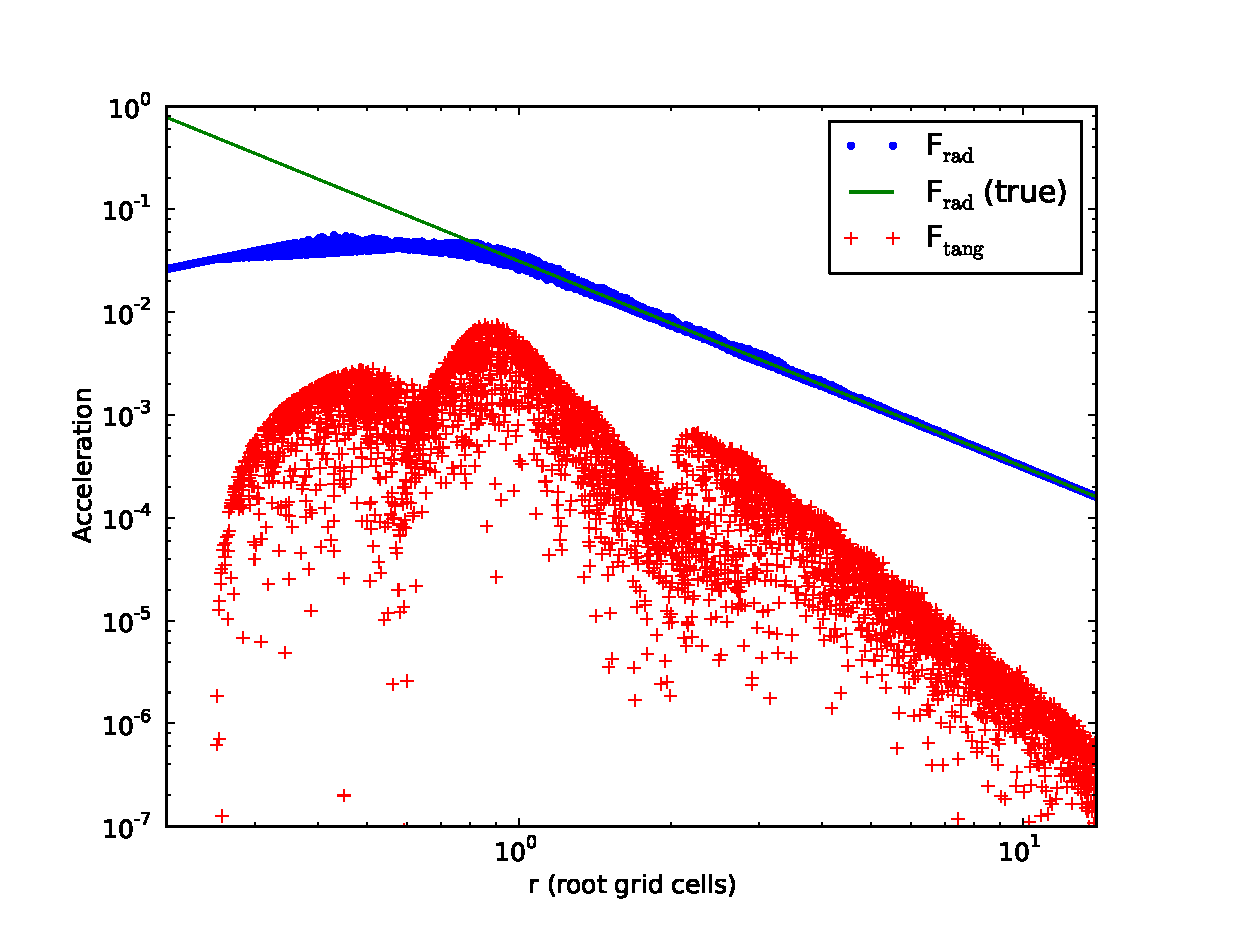
\includegraphics[width=0.6\textwidth]{figures/GravityTest.eps}
\caption{The radial and tangential accelerations measured around a point source placed in a static AMR grid.  The solid line shows the analytic radial profile.}
\label{fig.gravitytest}
\end{center}
\end{figure}
